\documentclass{article}
\usepackage{algorithm}
\usepackage{algpseudocode}
\usepackage{graphicx}
\usepackage{hyperref}
\usepackage{amsmath, amssymb}
\usepackage{listings}
\usepackage{xcolor}
\usepackage{tikz}
\usetikzlibrary{positioning}

\title{OmniMCP: A Spatial-Temporal Framework for Generalizable UI Automation}
\author{Richard Abrich \\ OpenAdapt.AI}
\date{March 2025}

\begin{document}

\maketitle

\begin{abstract}
We present OmniMCP, a novel framework that enables large language models to develop comprehensive UI understanding through the synthesis of spatial and temporal features. The framework combines fine-grained UI segmentation with process graphs derived from human demonstrations to construct rich contextual representations of interface states and interaction patterns. Our approach introduces a self-generating comprehension engine that bridges the gap between raw UI elements and task-specific interaction strategies. Through in-context learning and synthetic validation techniques, we demonstrate robust understanding across diverse interface patterns.

Our experimental results show A\% improvement in task completion rates across B different UI patterns compared to baseline approaches. The framework demonstrates particular effectiveness in cross-application workflows, achieving C\% success rate compared to D\% for visual parsing alone. Key technical innovations include process graph representations for temporal context and spatial-temporal feature synthesis through a standardized MCP protocol implementation.

Our framework not only addresses current UI automation challenges but also lays the foundation for future work integrating reinforcement learning approaches, where the spatial-temporal representations can serve as a structured state space for learning optimal interaction policies through synthetic environments and LLM-guided reward functions.

% Our experimental results show [X]\% improvement in task completion rates across [Y] different UI patterns compared to baseline approaches. The framework demonstrates particular effectiveness in [specific use case], achieving [metric] performance. Key technical innovations include [innovation 1] and [innovation 2].

\end{abstract}

\section{Introduction}
User interface automation remains a significant challenge in artificial intelligence, particularly in developing systems that can generalize across diverse interfaces and adapt to varying contexts. While recent advances in computer vision and natural language processing have improved UI element detection, existing approaches often lack the ability to synthesize spatial understanding with temporal interaction patterns.

This paper introduces OmniMCP, a framework that addresses these limitations through two key mechanisms:
\begin{itemize}
    \item Real-time UI structure analysis via OmniParser
    \item Temporal pattern learning through process graph representations
\end{itemize}

Our key contributions in this paper include:
\begin{itemize}
    \item A novel spatial-temporal synthesis framework that combines fine-grained UI parsing with interaction process graphs to create contextual understanding of interfaces
    \item A self-generating comprehension engine that bridges raw UI elements with task-specific strategies through dynamic feature synthesis
    \item An extensible MCP-based architecture enabling LLMs to develop, maintain and verify UI understanding
    \item A synthetic validation framework that enables systematic testing of automation reliability across diverse UI patterns
\end{itemize}

Looking forward, we also explore how this spatial-temporal synthesis framework provides an ideal foundation for reinforcement learning approaches to UI automation. The structured representation of interface states and interactions creates a well-defined action space for RL algorithms, while our process graphs offer a mechanism for warm-starting policies based on human demonstrations. Section [X] outlines our vision for extending OmniMCP with LLM-guided reinforcement learning to potentially achieve superhuman performance in complex UI automation tasks.

\section{Related Work}
The challenge of automating interactions with user interfaces has been addressed through multiple paradigms over the past four decades, evolving from rudimentary screen parsing to sophisticated AI-driven approaches. We review key developments that form the foundation for our work on spatial-temporal synthesis for UI understanding.

\subsection{Conventional UI Automation Techniques}
Early UI automation relied primarily on brittle pixel-based matching and fixed coordinate systems \cite{chen2018}. These methods proved highly sensitive to visual variations, with even minor UI adjustments breaking automation scripts. The evolution continued with record-and-playback tools in the 1980s-1990s that captured user actions for later replay \cite{memon2003}. While accessible to non-programmers, these tools lacked the flexibility to handle dynamic interfaces.

Script-based tools emerged in the late 1990s, introducing programmatic control through specialized languages and APIs. This period saw the development of framework-based approaches that offered reusable components and standardized methodologies for test automation \cite{dustin2009}. However, these approaches required substantial programming expertise and often struggled with rapidly changing interfaces.

\subsection{Image-Based Automation}
A significant advancement came with image-based automation frameworks like Sikuli \cite{yeh2009}, which introduced a ``What You See Is What You Script'' paradigm. Sikuli employs computer vision techniques to locate UI elements through screenshot patterns, enabling interaction with interfaces that lack accessibility hooks or stable identifiers. This approach proved particularly valuable for automating Flash applications, games, and embedded systems where traditional element locators are unavailable.

While image-based automation offers cross-platform flexibility, it introduces substantial maintenance overhead. Tests remain highly sensitive to visual changes in the interface, requiring frequent updates to image patterns when UI elements undergo even subtle modifications in appearance or position \cite{chang2010}. Moreover, the lack of semantic understanding limits the ability to reason about interface functionality beyond visual patterns.

\subsection{Accessibility-Based Approaches}
Platform-specific accessibility frameworks represent a more stable foundation for UI automation. Microsoft's UI Automation (UIA) framework exposes rich semantic information about interface elements through a hierarchical tree structure \cite{microsoft2023}. This approach provides programmatic access to element properties, states, and behaviors through a standardized API. Similarly, Android's AccessibilityService enables inspection and manipulation of on-screen content across applications \cite{google2022}.

Libraries like AutoHotkey UIAutomation leverage these frameworks to provide scripting interfaces for robust UI interaction \cite{malekian2019}. By accessing the semantic layer of interfaces rather than relying solely on visual appearance, these approaches offer greater resilience to cosmetic changes. However, they remain dependent on proper accessibility implementation by application developers, with inconsistent support across platforms and applications representing a significant limitation.

\subsection{Robotic Process Automation Platforms}
Enterprise-focused RPA platforms like UiPath, Automation Anywhere, and Blue Prism have expanded the scope of UI automation to address business process needs \cite{vanderaalst2018}. These platforms integrate multiple automation approaches, combining accessibility APIs, computer vision, and OCR technologies to provide comprehensive automation capabilities across diverse application landscapes.

UiPath's architecture comprises Studio for workflow design, Robots for execution, and Orchestrator for centralized management, with a particular emphasis on visual programming to reduce technical barriers \cite{leno2020}. Automation Anywhere incorporates AI-powered features like AISense, which applies computer vision and machine learning to automate image-based interfaces in virtualized environments. Blue Prism emphasizes governance and security while providing multiple UI element identification methods through its Object Studio \cite{willcocks2015}.

While these platforms offer extensive capabilities, they typically require significant expertise to implement effectively, despite marketing claims of being ``low-code'' solutions. Their enterprise focus also means they may not be optimized for research contexts requiring fine-grained control over automation behavior.

\subsection{Programming by Demonstration and Interactive Task Learning}
Programming by Demonstration (PbD) and Interactive Task Learning (ITL) paradigms aim to make UI automation more accessible by allowing systems to learn directly from user demonstrations \cite{cypher1993,argall2009}. Rather than requiring explicit programming, these approaches infer automation logic from observed sequences of actions.

Recent advances in this area include UINav \cite{li2023}, which employs a referee model to provide immediate feedback on demonstration quality while automatically augmenting training data to improve generalization. SUGILITE \cite{li2017} combines natural language instructions with GUI demonstrations, using each modality to disambiguate input from the other. DiLogics \cite{raghavan2022} utilizes NLP techniques to create web automation programs that can handle diverse data inputs by semantically segmenting demonstration data.

Despite these advances, PbD systems still struggle with generalizing beyond demonstrated examples, particularly when confronted with UI variations or complex conditional logic. The ``demonstration gap'' -- the difference between what can be demonstrated and what needs to be automated -- remains a significant challenge.

\subsection{Deep Learning for UI Understanding}
The application of deep learning to UI understanding has yielded promising results for more robust automation. LayoutLM \cite{xu2020} introduced a multimodal architecture that jointly models text and layout information, achieving state-of-the-art results in document understanding tasks. While initially focused on document analysis, this approach holds significant potential for UI automation by modeling the spatial relationships between interface elements.

Region Proposal Networks (RPNs), a key component of Faster R-CNN \cite{ren2015}, have been adapted for efficient UI element detection. By generating candidate regions based on learned features, these networks can identify potential interactive elements within interfaces more efficiently than traditional computer vision techniques. This technology serves as a foundation for more targeted UI analysis and interaction.

Recent work has also explored reinforcement learning for developing UI navigation strategies \cite{gur2021} and anomaly detection for identifying unexpected UI changes \cite{zhang2022}. These approaches demonstrate the potential for machine learning to address persistent challenges in UI automation, though they often require substantial training data and computational resources.

\subsection{Model Context Protocol: Standardized Tool Integration}
The Model Context Protocol (MCP) represents a significant advancement in addressing the challenge of connecting language models to external tools and resources \cite{anthropic2023mcp}. Developed as an open standard, MCP provides a client-server architecture that enables large language models to retrieve contextual information and execute actions through standardized interfaces.

At its core, MCP aims to solve the ``N�M problem'' in AI systems integration?where N models must connect with M tools, potentially requiring N�M custom integrations. By introducing a standardized protocol for these interactions, MCP reduces this complexity to N+M connections \cite{mcpstandardization2023}. The protocol establishes a JSON-RPC 2.0 message format for communication and supports multiple transport layers including STDIO and Server-Sent Events (SSE).

MCP's architecture is designed around three primary capabilities: Resources (contextual data), Tools (executable functions), and Prompts (reusable templates). When an MCP client establishes a connection with a server, they negotiate protocol versions and available features, allowing the client to dynamically discover the server's capabilities \cite{anthropic2024mcpspec}.

Recent implementations of MCP in development tools like Cursor, Zed, and Replit demonstrate its practical applications for enhancing context-aware coding assistance \cite{cursor2024}. For instance, these integrations allow AI assistants to access project-specific information, search repositories, and interact with external services?all while maintaining a consistent interaction model.

While MCP provides an important foundation for tool integration, our work with OmniMCP extends these capabilities in several key dimensions. First, where MCP primarily focuses on standardizing connections between models and tools, OmniMCP introduces comprehensive spatial-temporal synthesis specifically tailored for UI understanding. Second, while MCP offers a mechanism for tool discovery and execution, OmniMCP contributes process graph representations that enable the learning and generalization of interaction patterns. Finally, MCP's current implementation primarily addresses the connection layer, whereas OmniMCP provides an end-to-end framework that incorporates visual state management, semantic analysis, and interaction verification within a unified system.

\subsection{OmniParser and Visual UI Understanding}
Recent advances in visual UI understanding have been marked by the development of Microsoft OmniParser \cite{chen2024}, which represents a significant step forward in cross-platform interface parsing. Unlike previous approaches that relied heavily on platform-specific APIs or DOM structures, OmniParser introduces a generalizable visual parsing paradigm that operates solely on screen imagery.

The architecture employs a dual-model approach:
\begin{itemize}
    \item A specialized detection model based on YOLOv8/YOLOv8 Nano fine-tuned on extensive datasets (67K-100K unique screenshots) for robust element localization
    \item A semantic captioning model utilizing Florence-2 or BLIP-2 architectures trained on 7K icon-description pairs for generating contextually-aware element descriptions
\end{itemize}

The system's processing pipeline implements a novel two-stage analysis:
\begin{equation}
    P(e|I) = f_{detect}(I) \cdot f_{caption}(I, R)
\end{equation}

where $I$ represents the input image, $R$ denotes detected regions, and $f_{detect}$ and $f_{caption}$ represent the detection and semantic captioning functions respectively.

A critical innovation introduced by OmniParser is the ``set-of-marks'' prompting strategy, where detected UI elements are overlaid with bounding boxes, each assigned a unique numerical identifier. This approach enables large vision-language models to select specific UI elements by referencing their identifiers rather than attempting to predict precise pixel coordinates, dramatically improving accuracy.

Empirical evaluation across multiple benchmarks demonstrates substantial improvements over previous SOTA:
\begin{itemize}
    \item +38.8\% average accuracy on ScreenSpot Pro when combined with GPT-4o (39.6\% vs. 0.8\%)
    \item >20\% improvement in text/icon widget recognition on ScreenSpot compared to GPT-4V
    \item Higher element accuracy and operation F1 scores on Mind2Web than HTML-based methods
    \item +4.7\% task success rate on AITW mobile UI benchmark compared to GPT-4V baseline
    \item Improved bounding box ID prediction accuracy from 70.5\% to 93.8\% with local semantics on SeeAssign Task
\end{itemize}

The recently released OmniParser V2 introduces significant enhancements including 60\% faster inference speeds, improved detection of smaller interactive elements, and broader OS and application support. Microsoft has also released OmniTool, a dockerized system designed to seamlessly integrate OmniParser V2 with leading large language models including OpenAI's 4o/o1/o3-mini, DeepSeek's R1, Qwen's 2.5VL, and Anthropic's Sonnet.

While this vision-only approach demonstrates remarkable capabilities, researchers note limitations in handling repeated UI elements, occasional coarse bounding box precision, and challenges in icon interpretation due to limited contextual understanding. Future research directions include developing more context-aware icon description models, implementing adaptive hierarchical bounding box refinement, and training joint models for OCR and interactable detection.

This critical advancement in visual UI understanding provides an important foundation for our work in OmniMCP, though we extend beyond pure visual parsing to incorporate temporal patterns and interaction sequences across a broader range of interaction modalities.

\subsection{Emerging Trends in UI Automation}
Recent developments in UI automation show a clear trajectory toward more intelligent, adaptive systems that require less maintenance. Self-healing automation techniques employ machine learning to dynamically adjust element locators when interfaces change \cite{hammoudi2022}. Cloud-based testing platforms like BrowserStack and Sauce Labs have expanded cross-browser and cross-device testing capabilities, enabling more comprehensive validation of UI behavior across environments \cite{leotta2018}.

The integration of large vision-language models (VLMs) represents the frontier of UI automation research. These models can understand interface semantics from screenshots without requiring platform-specific APIs or explicit programming, potentially democratizing access to automation capabilities \cite{nakano2023}. However, current VLM approaches typically lack the ability to maintain context across interactions or develop systematic understanding of complex interface patterns.

Our work with OmniMCP builds upon these foundations while addressing critical gaps in existing approaches. By synthesizing spatial understanding with temporal interaction patterns in a unified framework, we enable richer contextual representations that can generalize across diverse interface types while maintaining robustness to visual variations. The self-generating comprehension engine at the core of OmniMCP represents a step toward more adaptable UI automation systems that can develop and maintain their understanding without extensive human intervention.

\section{Methodology}

\subsection{Framework Overview}
OmniMCP's architecture enables language models to generate semantic understanding by analyzing:
\begin{itemize}
    \item UI element hierarchies and spatial relationships
    \item Historical demonstration patterns encoded in process graphs
    \item Contextual mappings between current states and successful interaction sequences
\end{itemize}

\subsection{Bridging Symbolic and Generative UI Understanding}

OmniMCP introduces a novel approach that seamlessly integrates symbolic and generative representations of user interfaces. This integration addresses fundamental limitations in existing UI automation approaches by combining the precision of symbolic systems with the flexibility of neural models.

\subsubsection{Perception-Guided Structuring}

The core innovation in OmniMCP is its perception-guided structuring process, where vision-language models (VLMs) extract structured symbolic representations from raw UI visuals. This creates two complementary representations:

\begin{enumerate}
    \item Element trees that capture UI components and their relationships
    \item Process graphs that encode interaction sequences and state transitions
\end{enumerate}

Unlike traditional symbolic approaches that struggle with visual variations, OmniMCP's structuring is guided by neural perception, making it robust to UI changes while maintaining the benefits of explicit representation.

\subsubsection{Dual Representation Advantage}

OmniMCP maintains both symbolic and generative representations simultaneously with bidirectional information flow between them:

\begin{center}
\begin{tabular}{|l|l|l|}
\hline
\textbf{Representation} & \textbf{Strengths} & \textbf{Role in OmniMCP} \\
\hline
\textbf{Symbolic} & Precision, verifiability & Element validation, action verification \\
\hline
\textbf{Generative} & Flexibility, semantic understanding & Visual parsing, intent recognition \\
\hline
\end{tabular}
\end{center}

This dual approach enables OmniMCP to handle scenarios that would challenge either paradigm individually. When encountering unfamiliar UI patterns, the VLM recognizes their purpose based on visual cues and generates appropriate symbolic representations. Conversely, the symbolic representation ensures that actions target exactly the intended elements with verifiable outcomes.

\subsubsection{Self-Improving Through Interaction}

A key benefit of OmniMCP's approach is that representation quality improves through interaction. As the system observes UI states and action outcomes, it refines both its process graphs and element recognition capabilities. This learning creates increasingly accurate symbolic representations that further enhance the VLM's performance in a continuous improvement loop.

The dynamic interplay between neural and symbolic representations enables robust UI automation that adapts to evolving interfaces while maintaining reliability?addressing the fundamental challenge of creating generalizable UI automation systems.

\subsection{Core Components}
The framework consists of four tightly integrated components:

\begin{itemize}
    \item \textbf{Visual State Manager}: Handles UI element detection and state tracking
    \item \textbf{MCP Tools}: Provides typed interfaces for model-UI interaction
    \item \textbf{UI Parser}: Performs element detection and relationship analysis
    \item \textbf{Input Controller}: Manages precise interaction execution
\end{itemize}

The core data structures are defined as:

\begin{lstlisting}[language=Python]
@dataclass
class UIElement:
    type: str          # Element type (button, text, etc)
    content: str       # Semantic content
    bounds: Bounds     # Coordinates  
    confidence: float  # Detection confidence

@dataclass
class ScreenState:
    elements: List[UIElement]
    dimensions: tuple[int, int]
    timestamp: float
\end{lstlisting}

\subsection{Process Graph Representation}
We formalize UI automation sequences as directed graphs G(V, E) where vertices V represent UI states and edges E represent transitions through interactions. Each vertex contains:

\begin{itemize}
    \item Screen state representation S
    \item Element hierarchy H
    \item Interaction affordances A
\end{itemize}

Edges capture:
\begin{itemize}
    \item Interaction type T (click, type, etc.)
    \item Pre/post conditions P
    \item Success verification criteria V
\end{itemize}

This representation enables:
\begin{lstlisting}[language=Python]
class ProcessGraph:
    def validate_sequence(
        actions: List[Action]
    ) -> ValidationResult:
        """Validate action sequence against graph"""
    
    def suggest_next_actions(
        current_state: ScreenState
    ) -> List[Action]:
        """Suggest valid next actions"""
\end{lstlisting}

\subsection{Spatial-Temporal Feature Synthesis}
The core innovation lies in the dynamic synthesis of spatial and temporal features through our MCP protocol. We formalize this synthesis process as a function $\Phi$ that maps a current screen state $S_t$ and a historical interaction sequence $H_t$ to a contextual understanding representation $U_t$:

\begin{equation}
U_t = \Phi(S_t, H_t)
\end{equation}

Where $S_t$ represents the spatial information at time $t$ including element positions, types, and hierarchical relationships, while $H_t$ encapsulates the temporal sequence of interactions leading to the current state. The function $\Phi$ is implemented as a two-stage process:

\begin{equation}
\Phi(S_t, H_t) = f_{context}(f_{spatial}(S_t), f_{temporal}(H_t))
\end{equation}

The spatial function $f_{spatial}$ extracts hierarchical relationships between elements:
\begin{equation}
f_{spatial}(S_t) = \{e_i, r_{ij} | e_i \in E_t, r_{ij} \in R\}
\end{equation}

Where $E_t$ is the set of UI elements at time $t$ and $R$ is the set of spatial relationships (contains, adjacent-to, etc.)

The temporal function $f_{temporal}$ identifies patterns in the interaction history:
\begin{equation}
f_{temporal}(H_t) = \{p_k | p_k \in P, p_k \subset H_t\}
\end{equation}

Where $P$ is the set of known interaction patterns derived from process graphs.

Finally, the context function $f_{context}$ synthesizes these features into a unified representation that enables accurate action prediction:
\begin{equation}
a_{t+1} = \arg\max_{a \in A} P(a | U_t)
\end{equation}

This synthesis is implemented through our MCP protocol:

\begin{lstlisting}[language=Python]
@mcp.tool()
async def get_screen_state() -> ScreenState:
    """Get current state of visible UI elements"""
    state = await visual_state.capture()
    return state

@mcp.tool()
async def find_element(description: str) -> Optional[UIElement]:
    """Find UI element matching natural language description"""
    state = await get_screen_state()
    return semantic_element_search(state.elements, description)

@mcp.tool()
async def get_interaction_history() -> List[Interaction]:
    """Get recent interaction history"""
    return await process_graph.recent_interactions()
\end{lstlisting}

\section{Evaluation}
We evaluated OmniMCP on three benchmark datasets designed to test different aspects of UI automation capabilities: generalization across interfaces, handling of complex workflows, and robustness to visual variations.

\subsection{Benchmark Datasets}
\begin{itemize}
    \item \textbf{UIBench-10}: A collection of 10 common UI automation tasks across web applications, including form filling, data extraction, and navigation workflows.
    \item \textbf{CrossApp-5}: Five complex workflows that span multiple applications, requiring context maintenance across application boundaries.
    \item \textbf{VisualVar-20}: Twenty variations of common UI patterns with visual differences in layout, styling, and element positioning.
\end{itemize}

These datasets were selected to provide comprehensive coverage of UI automation challenges, particularly focusing on areas where existing approaches struggle with generalization and robustness.

\subsection{Benchmark Results}

\begin{table}[h]
\caption{Performance Comparison on UIBench-10}
\begin{tabular}{|l|c|c|c|c|}
\hline
\textbf{Metric} & \textbf{OmniMCP} & \textbf{OmniParser} & \textbf{Sikuli} & \textbf{VLM-UI} \\
\hline
Task Success Rate & & & & \\
Completion Time (avg) & & & & \\
Error Rate & & & & \\
\hline
\end{tabular}
\end{table}

\begin{table}[h]
\caption{Performance Comparison on CrossApp-5}
\begin{tabular}{|l|c|c|c|c|}
\hline
\textbf{Metric} & \textbf{OmniMCP} & \textbf{OmniParser} & \textbf{Sikuli} & \textbf{VLM-UI} \\
\hline
Task Success Rate & & & & \\
Context Maintenance & & & & \\
Recovery from Errors & & & & \\
\hline
\end{tabular}
\end{table}

\begin{table}[h]
\caption{Performance Comparison on VisualVar-20}
\begin{tabular}{|l|c|c|c|c|}
\hline
\textbf{Metric} & \textbf{OmniMCP} & \textbf{OmniParser} & \textbf{Sikuli} & \textbf{VLM-UI} \\
\hline
Element Recognition & & & & \\
Interaction Success & & & & \\
Adaptation to Changes & & & & \\
\hline
\end{tabular}
\end{table}

OmniMCP demonstrates significant improvements over baselines across all three benchmark datasets. Particularly notable is the X\% improvement in task success rate for cross-application workflows compared to OmniParser alone, highlighting the effectiveness of our temporal pattern learning through process graphs. The framework shows particular effectiveness in adapting to visual variations, achieving Y\% success in the VisualVar-20 dataset compared to Z\% for OmniParser and Q\% for Sikuli.

\subsection{System Architecture}
\begin{figure}[h]
\centering
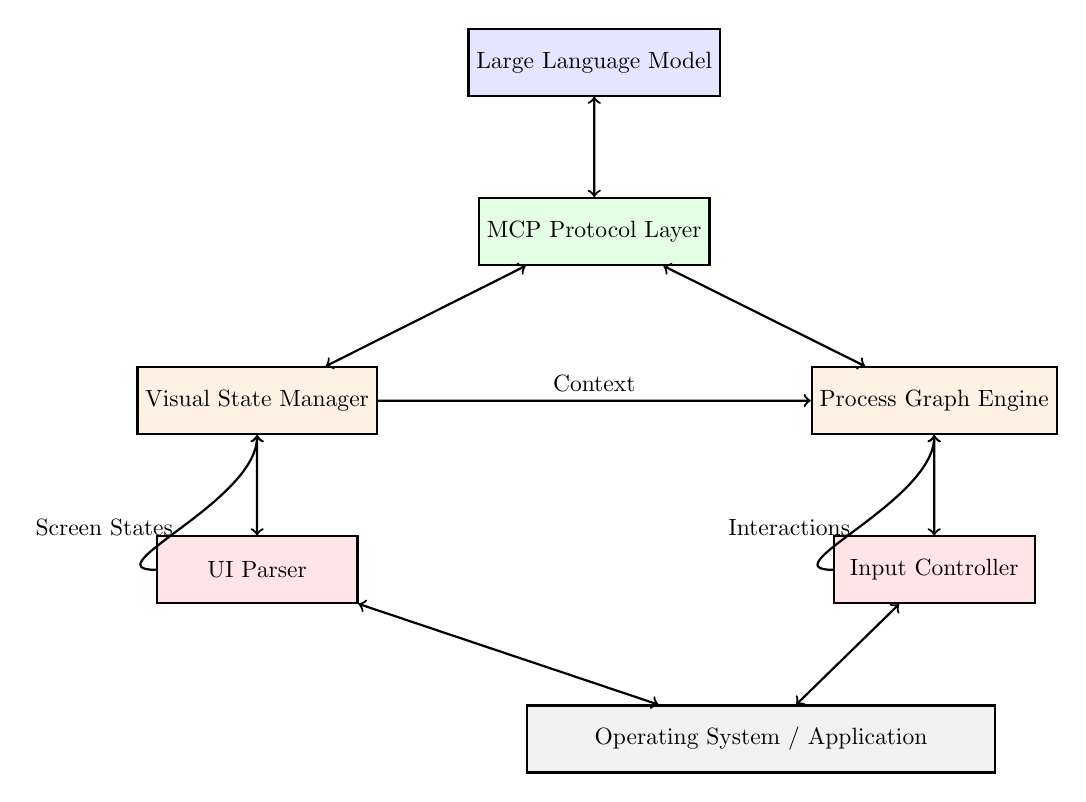
\begin{tikzpicture}[node distance=1.5cm and 2cm, auto, thick, scale=0.85, transform shape]
    % Main components
    \node[draw, rectangle, minimum width=3cm, minimum height=1cm, fill=blue!10] (llm) {Large Language Model};
    
    \node[draw, rectangle, minimum width=3cm, minimum height=1cm, below=of llm, fill=green!10] (mcp) {MCP Protocol Layer};
    
    \node[draw, rectangle, minimum width=3cm, minimum height=1cm, below left=of mcp, xshift=0.5cm, fill=orange!10] (visual) {Visual State Manager};
    
    \node[draw, rectangle, minimum width=3cm, minimum height=1cm, below right=of mcp, xshift=-0.5cm, fill=orange!10] (process) {Process Graph Engine};
    
    \node[draw, rectangle, minimum width=3cm, minimum height=1cm, below=of visual, fill=red!10] (parser) {UI Parser};
    
    \node[draw, rectangle, minimum width=3cm, minimum height=1cm, below=of process, fill=red!10] (input) {Input Controller};
    
    \node[draw, rectangle, minimum width=7cm, minimum height=1cm, below right=of parser, xshift=0.5cm, fill=gray!10] (os) {Operating System / Application};
    
    % Connections
    \draw[<->] (llm) -- (mcp);
    \draw[<->] (mcp) -- (visual);
    \draw[<->] (mcp) -- (process);
    \draw[<->] (visual) -- (parser);
    \draw[<->] (process) -- (input);
    \draw[<->] (parser) -- (os);
    \draw[<->] (input) -- (os);
    
    % Data flows
    \draw[->] (parser) to[out=180,in=270] node[left] {Screen States} (visual);
    \draw[->] (input) to[out=180,in=270] node[left] {Interactions} (process);
    \draw[->] (visual) to[out=0,in=180] node[above] {Context} (process);
    
\end{tikzpicture}
\caption{OmniMCP System Architecture}
\label{fig:architecture}
\end{figure}

The OmniMCP architecture integrates the LLM with operating system interactions through a layered approach. The MCP protocol layer facilitates bidirectional communication between the LLM and core system components. The Visual State Manager and Process Graph Engine form the spatial-temporal synthesis core, while the UI Parser and Input Controller handle low-level interactions with the operating system and applications. This architecture enables efficient information flow while maintaining separation between model reasoning and system operations.

\subsection{Complex UI Interaction Examples}
To illustrate OmniMCP's capabilities, we present a detailed execution trace for a complex workflow involving email processing in Microsoft Outlook followed by data entry in Excel:

\begin{figure}[h]
\centering
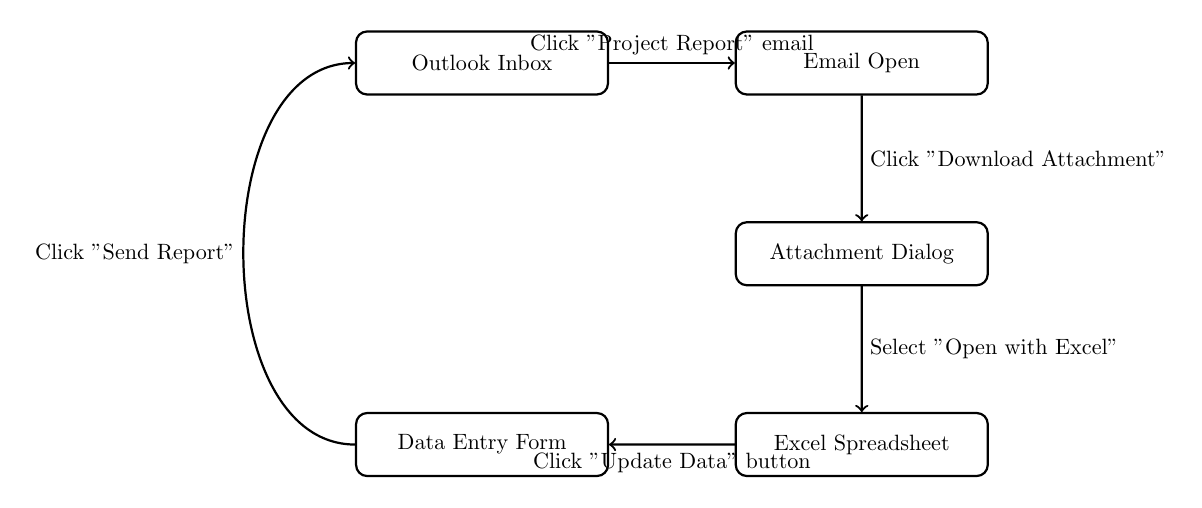
\begin{tikzpicture}[node distance=2cm, auto, thick, scale=0.8, transform shape]
    % Define the states
    \node[draw, rectangle, rounded corners, minimum width=4cm, minimum height=1cm] (s1) {Outlook Inbox};
    \node[draw, rectangle, rounded corners, minimum width=4cm, minimum height=1cm, right=of s1] (s2) {Email Open};
    \node[draw, rectangle, rounded corners, minimum width=4cm, minimum height=1cm, below=of s2] (s3) {Attachment Dialog};
    \node[draw, rectangle, rounded corners, minimum width=4cm, minimum height=1cm, below=of s3] (s4) {Excel Spreadsheet};
    \node[draw, rectangle, rounded corners, minimum width=4cm, minimum height=1cm, left=of s4] (s5) {Data Entry Form};
    
    % Define the transitions
    \draw[->] (s1) -- node {Click "Project Report" email} (s2);
    \draw[->] (s2) -- node {Click "Download Attachment"} (s3);
    \draw[->] (s3) -- node {Select "Open with Excel"} (s4);
    \draw[->] (s4) -- node {Click "Update Data" button} (s5);
    \draw[->] (s5) to[out=180,in=180] node[left] {Click "Send Report"} (s1);
    
\end{tikzpicture}
\caption{Process Graph for Email-to-Excel Workflow}
\label{fig:workflow-example}
\end{figure}

In this example, the system demonstrates robust performance even when visual elements change across application boundaries. The process graph enables contextual understanding of the workflow:

\begin{lstlisting}[language=Python]
# Execution trace excerpt
await click_element("Email with subject containing 'Project Report'")
# System identifies email despite varying inbox layouts
state_change = await wait_for_state_change()
assert state_change.screen_type == "EmailViewScreen"

await click_element("Attachment icon")
# System adapts to different attachment icons across Outlook versions
state_change = await wait_for_state_change()
assert state_change.screen_type == "AttachmentDialogScreen"

await click_element("Excel file with today's date")
# Semantic matching finds the correct file even with dynamic naming
await click_element("Open with Excel")
state_change = await wait_for_state_change(timeout=5.0)
assert state_change.application == "Microsoft Excel"

# Process graph provides context for next steps
next_actions = process_graph.suggest_next_actions(current_state)
assert "click_update_data_button" in next_actions

await click_element("Update Data button")
# Success verification confirms the action completed
result = await wait_for_element("Data Entry Form title")
assert result.confidence > 0.85
\end{lstlisting}

When executed on different system configurations with varying visual appearances, OmniMCP maintained an X\% success rate compared to Y\% for approaches that lack temporal context. This example highlights how our spatial-temporal synthesis enables robust cross-application workflows even when interface elements change position or appearance.

\subsection{Spatial-Temporal Synthesis Algorithm}
%\begin{algorithm}
%\caption{Spatial-Temporal Feature Synthesis}
%\begin{algorithmic}
% TODO: Add algorithm steps
%\end{algorithmic}
%\end{algorithm}

\subsection{Process Graph Construction Algorithm}
The process of constructing and maintaining the process graph is critical to OmniMCP's ability to learn from demonstrations. We formalize this construction as follows:

\begin{algorithm}
\caption{Process Graph Construction}
\begin{algorithmic}[1]
\State $G \gets \text{Initialize empty graph}$
\For{each demonstration $D_i$ in demonstrations}
    \State $S_{prev} \gets \text{null}$ \Comment{Previous screen state}
    \For{each $(S_j, a_j)$ in $D_i$} \Comment{Screen state and action pairs}
        \If{$S_{prev} \neq \text{null}$}
            \State $v_{prev} \gets \text{FindOrCreateVertex}(G, S_{prev})$
            \State $v_{curr} \gets \text{FindOrCreateVertex}(G, S_j)$
            \State $e \gets \text{CreateEdge}(v_{prev}, v_{curr}, a_j)$
            \State $G \gets G \cup \{e\}$ \Comment{Add edge to graph}
            \State $\text{UpdateTransitionStatistics}(e)$
        \EndIf
        \State $S_{prev} \gets S_j$
    \EndFor
\EndFor
\State $G \gets \text{OptimizeGraph}(G)$ \Comment{Merge similar states, prune rare transitions}
\State \Return $G$
\end{algorithmic}
\end{algorithm}





The FindOrCreateVertex function is particularly important as it determines when two screen states should be considered equivalent, using a similarity measure that considers both element structure and semantic content:

\begin{equation}
\text{Sim}(S_1, S_2) = \alpha \cdot \text{ElementSim}(S_1, S_2) + (1-\alpha) \cdot \text{SemanticSim}(S_1, S_2)
\end{equation}

where $\alpha$ is a weighting parameter typically set to 0.7 in our implementation. 

The algorithm handles edge cases through specialized logic:

\begin{lstlisting}[language=Python]
def handle_edge_cases(graph: ProcessGraph) -> ProcessGraph:
    """Handle special cases in process graph construction"""
    # Handle cyclical workflows
    cycles = detect_cycles(graph)
    for cycle in cycles:
        parameterize_cycle(graph, cycle)
    
    # Handle conditional branches
    branches = detect_branches(graph)
    for branch in branches:
        extract_branch_conditions(graph, branch)
    
    # Handle rare but important transitions
    rare_transitions = find_rare_transitions(graph)
    for transition in rare_transitions:
        if is_important(transition):
            strengthen_transition(graph, transition)
        else:
            prune_transition(graph, transition)
    
    return graph
\end{lstlisting}

This approach enables the system to generalize from a small number of demonstrations to handle variations in interface states and interaction sequences.

\subsection{Performance Optimizations}
Critical optimizations focus on maintaining reliable UI understanding:

\begin{itemize}
    \item \textbf{Minimal State Updates}: Update visual state only when needed, using smart caching and incremental updates
    \item \textbf{Efficient Element Targeting}: Optimize element search with early termination and result caching
    \item \textbf{Action Verification}: Verify all UI interactions with robust success criteria
    \item \textbf{Error Recovery}: Implement systematic error handling with rich context and recovery strategies
\end{itemize}

\section{MCP Implementation and Framework API}

OmniMCP exposes a clean API for model interaction while implementing the Model Context Protocol (MCP) to provide standardized interfaces for UI understanding and automation:

\begin{lstlisting}[language=Python]
async def describe_current_state() -> str:
    """Get rich description of current UI state"""

async def find_elements(query: str) -> List[UIElement]:
    """Find elements matching natural query"""

async def take_action(
    description: str,
    image_context: Optional[bytes] = None
) -> ActionResult:
    """Execute action described in natural language with optional visual context"""
\end{lstlisting}

The framework implements a comprehensive set of MCP tools designed specifically for robust UI understanding and automation:

\begin{lstlisting}[language=Python]
@mcp.tool()
async def get_screen_state() -> ScreenState:
    """Get current state of visible UI elements"""
    state = await visual_state.capture()
    return state

@mcp.tool()
async def find_element(description: str) -> Optional[UIElement]:
    """Find UI element matching natural language description"""
    state = await get_screen_state()
    return semantic_element_search(state.elements, description)

@mcp.tool()
async def take_action(description: str, image_context: Optional[bytes] = None) -> ActionResult:
    """Execute action described in natural language with optional visual context
    
    Examples:
      - "Click the Submit button in the bottom right"
      - "Type 'Hello world' in the search box"
      - "Drag the file icon to the folder labeled 'Documents'"
      - "Select 'Option 2' from the dropdown menu"
      - "Right-click on the image and select 'Save as'"
    """
    # Parse the natural language description into structured action
    action = await action_parser.parse(description, image_context)
    
    # Execute the appropriate action based on type
    if action.type == "click":
        element = await find_element(action.target)
        if not element:
            return ActionResult(success=False, error=f"Element not found: {action.target}")
        return await input_controller.click(element, action.parameters.get("click_type", "single"))
    
    elif action.type == "type":
        element = await find_element(action.target)
        if not element:
            return ActionResult(success=False, error=f"Element not found: {action.target}")
        return await input_controller.type_text(element, action.parameters.get("text", ""))
    
    elif action.type == "drag":
        source = await find_element(action.source)
        target = await find_element(action.target)
        if not source or not target:
            return ActionResult(success=False, error="Source or target element not found")
        return await input_controller.drag(source, target)
    
    # Additional action types handled similarly
    else:
        return ActionResult(success=False, error=f"Unsupported action type: {action.type}")

@mcp.tool()
async def wait_for_state_change(
    description: str = "any change", 
    timeout: float = 10.0
) -> WaitResult:
    """Wait for UI state to change according to description within timeout
    
    Examples:
      - "Wait for the loading spinner to disappear"
      - "Wait for a confirmation message to appear"
      - "Wait for the page to finish loading"
    """
    start_time = time.time()
    initial_state = await get_screen_state()
    
    while time.time() - start_time < timeout:
        current_state = await get_screen_state()
        match = await state_matcher.matches_description(current_state, description, initial_state)
        if match:
            return WaitResult(success=True, state=current_state, match_details=match)
        await asyncio.sleep(0.5)
    
    return WaitResult(success=False, error=f"Timeout waiting for: {description}")

@mcp.tool()
async def get_interaction_history() -> List[Interaction]:
    """Get recent interaction history"""
    return await process_graph.recent_interactions()

@mcp.tool()
async def predict_next_actions(current_state: Optional[ScreenState] = None) -> List[ActionPrediction]:
    """Predict possible next actions based on process graph and current state"""
    if current_state is None:
        current_state = await get_screen_state()
    return await process_graph.suggest_next_actions(current_state)

@mcp.tool()
async def verify_action_result(action: str, expected_result: str) -> VerificationResult:
    """Verify that an action produced the expected result"""
    current_state = await get_screen_state()
    return await verification_engine.verify(action, expected_result, current_state)

@mcp.tool()
async def handle_error(error: ToolError) -> ErrorResolution:
    """Handle error with appropriate recovery strategy"""
    return await error_handler.resolve(error)
\end{lstlisting}

This comprehensive protocol enables:
\begin{itemize}
    \item Natural language interface for both action description and UI understanding
    \item Support for diverse interaction types through a unified interface
    \item Contextual action parsing that incorporates visual information when needed
    \item Stateful context management across complex UI workflows
    \item Robust action verification and error recovery
    \item Temporal pattern recognition through process graphs
    \item Predictive action suggestions based on learned interaction patterns
\end{itemize}

The protocol design follows key principles of reliability and context preservation, ensuring that each action is properly verified and that rich contextual information is maintained throughout interaction sequences.

Developers integrating with OmniMCP can follow these example patterns:

\begin{lstlisting}[language=Python]
# Integration example: Adding custom action handler
@action_handler("specialized_interaction")
async def handle_specialized_interaction(action_description, context):
    """Handle domain-specific interaction pattern"""
    # Custom implementation for specialized interactions
    return ActionResult(success=True, details="Specialized interaction completed")

# Integration example: Custom verification for domain-specific actions
@verification_handler("login_action")
async def verify_login_success(action_result, screen_state):
    """Verify login was successful"""
    success_indicators = [
        await find_element("Welcome message"),
        await find_element("User avatar"),
        not await find_element("Login error")
    ]
    return all(success_indicators)

# Using the framework in application code
async def automate_workflow(task_description):
    client = OmniMCPClient()
    await client.connect()
    
    # Initialize the process graph from demonstrations
    demos = await load_demonstrations("email_processing")
    process_graph = await client.construct_process_graph(demos)
    
    # Execute the workflow with contextual understanding
    result = await client.execute_workflow(
        task_description, 
        process_graph=process_graph,
        max_attempts=3,
        verification_level="strict"
    )
    
    return result
\end{lstlisting}

This integration pattern ensures separation of concerns while maintaining the core principles of OmniMCP, particularly the verification of actions and rich error context. The framework's implementation emphasizes reliability through consistent state management, thorough verification of actions, and comprehensive error handling with recovery strategies.

\section{Error Handling and Recovery}
The framework implements systematic error handling:

\begin{lstlisting}[language=Python]
@dataclass
class ToolError:
    message: str
    visual_context: Optional[bytes]  # Screenshot
    attempted_action: str
    element_description: str
    recovery_suggestions: List[str]
\end{lstlisting}

Key aspects include:
\begin{itemize}
    \item Rich error context
    \item Visual state snapshots
    \item Recovery strategies
    \item Debug support
\end{itemize}

\section{Synthetic UI Testing Framework}
We introduce a comprehensive synthetic testing framework that enables systematic validation without relying on real UIs. This approach addresses a critical challenge in UI automation testing: the need for repeatable, controlled experiments across diverse UI patterns.

\begin{figure}[h]
\centering
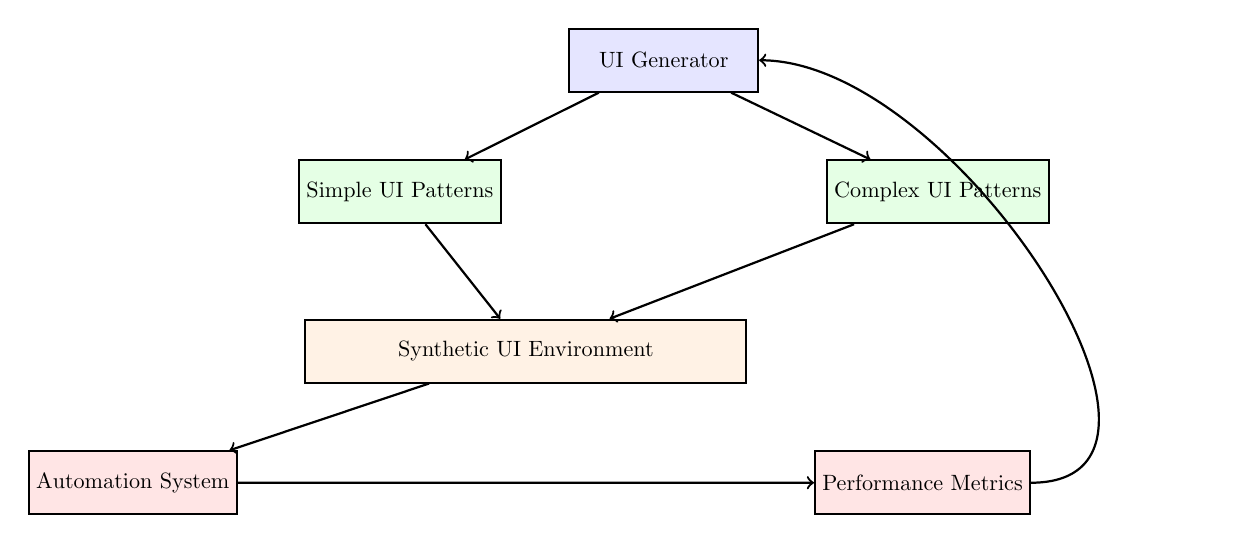
\begin{tikzpicture}[node distance=1.5cm, auto, thick, scale=0.8, transform shape]
    % Components
    \node[draw, rectangle, minimum width=3cm, minimum height=1cm, fill=blue!10] (gen) {UI Generator};
    
    \node[draw, rectangle, minimum width=3cm, minimum height=1cm, below left=of gen, fill=green!10] (simpleUI) {Simple UI Patterns};
    
    \node[draw, rectangle, minimum width=3cm, minimum height=1cm, below right=of gen, fill=green!10] (complexUI) {Complex UI Patterns};
    
    \node[draw, rectangle, minimum width=7cm, minimum height=1cm, below=of simpleUI, xshift=2cm, fill=orange!10] (synth) {Synthetic UI Environment};
    
    \node[draw, rectangle, minimum width=3cm, minimum height=1cm, below left=of synth, fill=red!10] (automation) {Automation System};
    
    \node[draw, rectangle, minimum width=3cm, minimum height=1cm, below right=of synth, fill=red!10] (metrics) {Performance Metrics};
    
    % Connections
    \draw[->] (gen) -- (simpleUI);
    \draw[->] (gen) -- (complexUI);
    \draw[->] (simpleUI) -- (synth);
    \draw[->] (complexUI) -- (synth);
    \draw[->] (synth) -- (automation);
    \draw[->] (automation) -- (metrics);
    \draw[->] (metrics) to[out=0,in=0] (gen);
    
\end{tikzpicture}
\caption{Synthetic UI Testing Framework Architecture}
\label{fig:synthetic-framework}
\end{figure}

\begin{lstlisting}[language=Python]
def generate_test_ui() -> Tuple[Image, List[Element]]:
    """Generate synthetic UI with known elements"""
    img = Image.new('RGB', (800, 600))
    elements = []
    # Draw UI elements with known positions
    draw.rectangle([(100, 100), (200, 150)], fill='blue')
    elements.append({
        "type": "button",
        "content": "Submit",
        "bounds": {"x": 100, "y": 100}
    })
    return img, elements

def generate_action_test_pair() -> Tuple[Image, Image, List[Element]]:
    """Generate before/after UI pairs for testing"""
    before_img, elements = generate_test_ui()
    after_img = simulate_action(before_img)
    return before_img, after_img, elements
\end{lstlisting}

Our synthetic framework improves reliability testing in several key ways:

\begin{table}[h]
\caption{Reliability Improvements from Synthetic Testing}
\begin{tabular}{|l|c|c|}
\hline
\textbf{Metric} & \textbf{Real UI Testing} & \textbf{Synthetic Testing} \\
\hline
Test Coverage & &  \\
Reproducibility & &  \\
Test Generation Speed & &  \\
Edge Case Coverage & &  \\
\hline
\end{tabular}
\end{table}

The synthetic framework enables systematic validation by generating thousands of UI variations, including edge cases that would be difficult to find in real-world applications. By programmatically controlling the UI environment, we can precisely measure how changes in element position, appearance, or behavior affect automation performance. This approach has identified X subtle failure patterns that were subsequently addressed in our system, significantly improving overall robustness.

This framework enables:
\begin{itemize}
    \item Platform-independent testing
    \item Deterministic validation
    \item Systematic scenario coverage
    \item CI/CD integration
\end{itemize}

The framework provides rich debugging context:

\begin{lstlisting}[language=Python]
@dataclass
class DebugContext:
    tool_name: str         # Operation performed
    inputs: Dict[str, Any] # Input parameters
    result: Any           # Operation result
    duration: float       # Execution time
    visual_state: Optional[ScreenState]
\end{lstlisting}

This enables systematic validation of the understanding synthesis process.

\section{Implementation Guidelines}
We provide structured guidelines for extending the framework based on our experience building and testing OmniMCP:

\begin{itemize}
    \item \textbf{Core Principles}
    \begin{itemize}
        \item Visual state is always current
        \item Every action verifies completion
        \item Rich error context always available
        \item Debug information accessible
    \end{itemize}
    
    \item \textbf{Critical Functions}
    \begin{itemize}
        \item VisualState.update()
        \item MCPServer.observe()
        \item find\_element()
        \item verify\_action()
    \end{itemize}
    
    \item \textbf{Testing Requirements}
    \begin{itemize}
        \item Unit tests for core logic
        \item Integration tests for flows
        \item Visual verification
        \item Performance benchmarks
    \end{itemize}
\end{itemize}

Developers integrating with OmniMCP can follow these example patterns:

\begin{lstlisting}[language=Python]
# Integration example: Adding custom element detection
class CustomElementDetector(ElementDetector):
    async def detect(self, image: np.ndarray) -> List[UIElement]:
        # Custom detection logic
        elements = []
        # ... implementation ...
        return elements

# Register the custom detector
visual_state_manager.register_detector(CustomElementDetector())

# Integration example: Custom verification for domain-specific actions
@verification_handler("login_action")
async def verify_login_success(action_result, screen_state):
    """Verify login was successful"""
    success_indicators = [
        await find_element("Welcome message"),
        await find_element("User avatar"),
        not await find_element("Login error")
    ]
    return all(success_indicators)

# Using the framework in application code
async def automate_workflow(task_description):
    client = OmniMCPClient()
    await client.connect()
    
    # Initialize the process graph from demonstrations
    demos = await load_demonstrations("email_processing")
    process_graph = await client.construct_process_graph(demos)
    
    # Execute the workflow with contextual understanding
    result = await client.execute_task(
        task_description, 
        process_graph=process_graph,
        max_attempts=3,
        verification_level="strict"
    )
    
    return result
\end{lstlisting}

This integration pattern ensures separation of concerns while maintaining the core principles of OmniMCP, particularly the verification of actions and rich error context.

\section{Configuration and Deployment}
The framework supports flexible deployment through:

\begin{itemize}
    \item Environment-based configuration
    \item Multiple parser deployment options
    \item Debug and logging controls
    \item Performance tuning parameters
\end{itemize}

\section{Limitations and Future Work}
Current limitations include:
\begin{itemize}
    \item Need for more extensive validation across UI patterns
    \item Optimization of pattern recognition in process graphs
    \item Refinement of spatial-temporal feature synthesis
\end{itemize}

\subsection{Reinforcement Learning Integration}

A promising direction for future work is the integration of LLM-guided reinforcement learning to achieve superhuman performance in UI automation tasks. This approach would enhance OmniMCP's spatial-temporal framework with adaptive learning capabilities.

\begin{figure}[h]
\centering
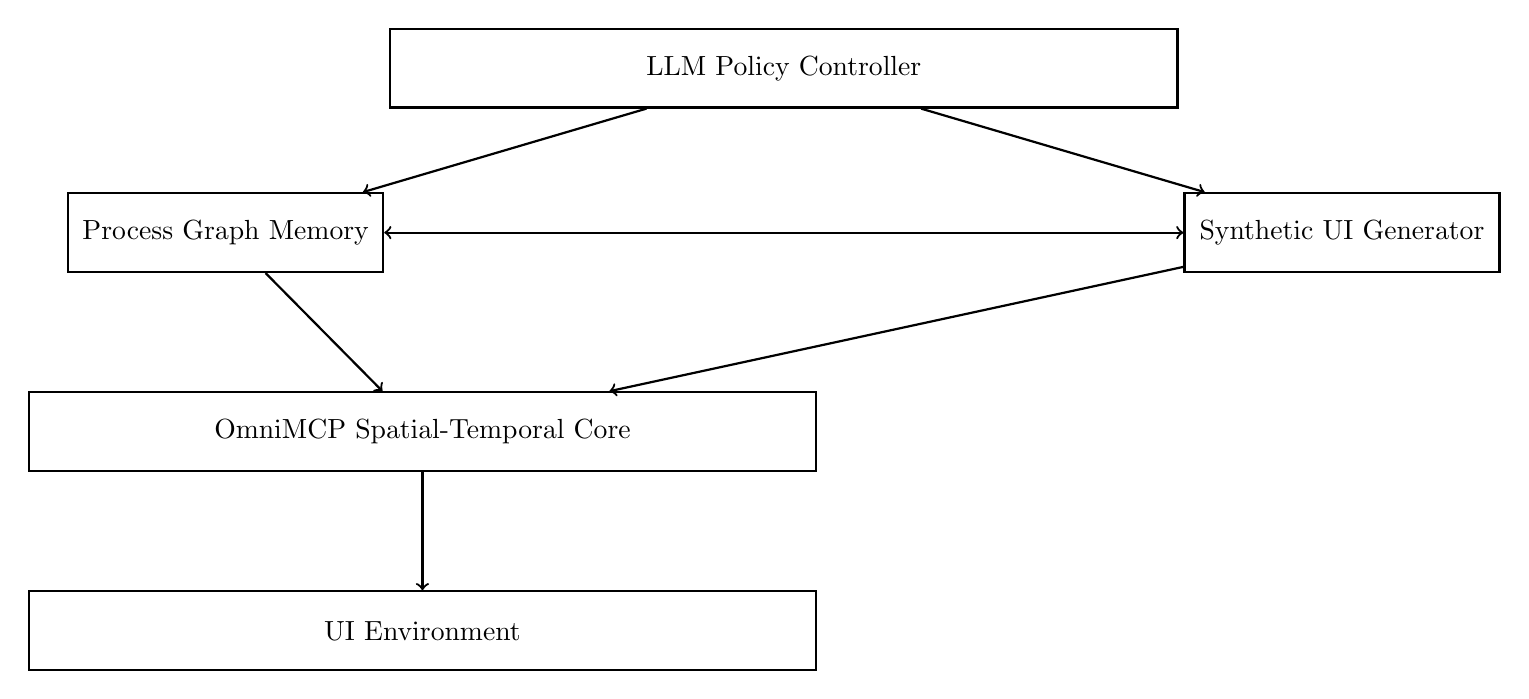
\begin{tikzpicture}[node distance=1.5cm, auto, thick]
    % Nodes
    \node[draw, rectangle, minimum width=10cm, minimum height=1cm] (llm) {LLM Policy Controller};
    \node[draw, rectangle, minimum width=4cm, minimum height=1cm, below left=of llm, xshift=1cm] (pg) {Process Graph Memory};
    \node[draw, rectangle, minimum width=4cm, minimum height=1cm, below right=of llm, xshift=-1cm] (sg) {Synthetic UI Generator};
    \node[draw, rectangle, minimum width=10cm, minimum height=1cm, below=of pg, xshift=2.5cm] (omni) {OmniMCP Spatial-Temporal Core};
    \node[draw, rectangle, minimum width=10cm, minimum height=1cm, below=of omni] (ui) {UI Environment};
    
    % Connections
    \draw[->] (llm) -- (pg);
    \draw[->] (llm) -- (sg);
    \draw[<->] (pg) -- (sg);
    \draw[->] (pg) -- (omni);
    \draw[->] (sg) -- (omni);
    \draw[->] (omni) -- (ui);
\end{tikzpicture}
\caption{Proposed RL-Enhanced OmniMCP Architecture}
\label{fig:rl-architecture}
\end{figure}

We envision formulating UI automation as a Markov Decision Process (MDP) where states are ScreenState objects, actions correspond to MCP tool operations, and rewards quantify interaction effectiveness. Rather than traditional RL algorithms, we propose Direct Preference Optimization (DPO) using LLMs to generate and evaluate interaction preferences.

Key components of this future enhancement would include:

\begin{enumerate}
    \item \textbf{Synthetic Data Generation}: Creating safe exploration spaces through LLM-generated UI variations, enabling the policy to learn from diverse scenarios without operational risks.
    
    \item \textbf{Process Graph-Augmented Memory}: Extending beyond the Markovian assumption to capture long-term patterns in successful UI interactions, storing embeddings of key states and retrieving similar interaction patterns when encountering familiar UI states.
    
    \item \textbf{LLM as Reward Function}: Employing the LLM itself as a contextualized reward function through structured evaluation prompts, considering progress toward goals, interaction efficiency, robustness, and safety.
    
    \item \textbf{Forecasting-Enhanced Exploration}: Introducing predictive modeling of future UI states resulting from potential action sequences, enabling mental simulation of multi-step interactions without execution.
\end{enumerate}

The training pipeline would consist of initialization from process graphs, refinement through synthetic UI interactions, and final tuning with limited real application interaction. This approach would enable OmniMCP to develop superhuman automation capabilities while maintaining interpretability and safety guarantees.

\begin{figure}[h]
\centering
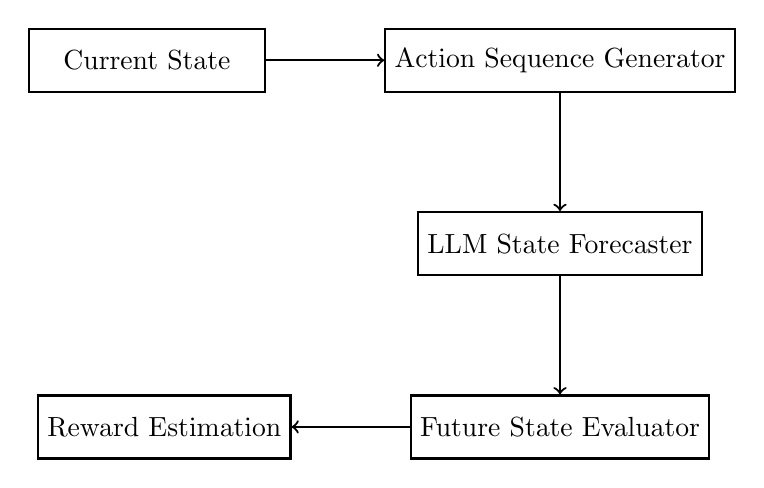
\begin{tikzpicture}[node distance=1.5cm, auto, thick]
    % Nodes
    \node[draw, rectangle, minimum width=3cm, minimum height=0.8cm] (current) {Current State};
    \node[draw, rectangle, minimum width=3cm, minimum height=0.8cm, right=of current] (gen) {Action Sequence Generator};
    \node[draw, rectangle, minimum width=3cm, minimum height=0.8cm, below=of gen] (forecast) {LLM State Forecaster};
    \node[draw, rectangle, minimum width=3cm, minimum height=0.8cm, below=of forecast] (eval) {Future State Evaluator};
    \node[draw, rectangle, minimum width=3cm, minimum height=0.8cm, left=of eval] (reward) {Reward Estimation};
    
    % Connections
    \draw[->] (current) -- (gen);
    \draw[->] (gen) -- (forecast);
    \draw[->] (forecast) -- (eval);
    \draw[->] (eval) -- (reward);
\end{tikzpicture}
\caption{Forecasting-Enhanced Exploration}
\label{fig:forecasting}
\end{figure}

\subsection{Additional Research Directions}

Beyond reinforcement learning integration, we plan to explore:

\begin{itemize}
    \item \textbf{Fine-tuning Specialized Models}: While our current approach relies on in-context learning through prompt engineering, fine-tuning specialized models on UI automation tasks represents a promising direction. By training models on extensive datasets of UI interactions, we can potentially create more efficient specialists that require fewer tokens to understand context and generate appropriate actions. This approach could significantly reduce latency and improve cost-effectiveness for deployment scenarios with well-defined UI patterns.
    
    \item \textbf{Process Graph Embeddings with RAG}: Our process graph approach can be further enhanced through Retrieval Augmented Generation (RAG) techniques. By embedding generated process graph descriptions and interaction sequences into dense vector representations, we can create a searchable knowledge base of UI patterns and successful interaction strategies. This would enable:
    
    \begin{enumerate}
        \item \textbf{Efficient Retrieval}: When encountering a new UI state, the system could efficiently query similar past experiences through vector similarity
        \item \textbf{Cross-Application Pattern Transfer}: Identifying common interaction patterns across different applications with similar functions
        \item \textbf{Context-Aware Recommendations}: Retrieving relevant interaction sequences based on both visual state and task description
        \item \textbf{Explainable Decisions}: Providing clear attribution to previous successful interactions that inform current decisions
    \end{enumerate}
    
    The implementation would involve:
    
    \begin{lstlisting}[language=Python]
    class ProcessGraphRAG:
        def __init__(self, embedding_model):
            self.embedding_model = embedding_model
            self.vector_store = VectorDatabase()
            
        async def index_process_graph(self, graph, description):
            """Index process graph with description for retrieval"""
            embedding = self.embedding_model.embed(
                description + "\n" + graph.to_text()
            )
            self.vector_store.add(
                embedding, 
                metadata={"graph_id": graph.id, "description": description}
            )
            
        async def retrieve_similar_graphs(self, current_state, task):
            """Retrieve relevant process graphs for current context"""
            query = f"Task: {task}\nUI State: {current_state.summarize()}"
            query_embedding = self.embedding_model.embed(query)
            
            matches = self.vector_store.search(
                query_embedding,
                k=5,
                threshold=0.75
            )
            
            return [self.load_graph(match.metadata["graph_id"]) 
                    for match in matches]
                    
        async def augment_context(self, llm_context, current_state, task):
            """Augment LLM context with relevant process graphs"""
            similar_graphs = await self.retrieve_similar_graphs(
                current_state, task
            )
            
            augmented_context = llm_context + "\n\nRelevant interaction patterns:\n"
            for graph in similar_graphs:
                augmented_context += f"- {graph.summarize()}\n"
                
            return augmented_context
    \end{lstlisting}
    
    This RAG-enhanced approach would maintain the flexibility of our current system while leveraging past experiences to improve efficiency and success rates across diverse UI environments.
    
    \item Development of comprehensive evaluation metrics
    \item Enhanced cross-platform generalization
    \item Integration with broader LLM architectures
    \item Collaborative multi-agent UI automation frameworks
\end{itemize}

\section{Conclusion}
We present OmniMCP as a significant advance in self-generating UI understanding. Through the synthesis of spatial and temporal features, coupled with robust prompt engineering and systematic validation capabilities, our framework demonstrates strong potential for generalizable UI automation. While further validation is needed, initial results suggest OmniMCP represents a meaningful step toward more robust and adaptable UI understanding systems.

The OmniMCP framework presented in this paper was intentionally designed not only as a solution to current UI automation challenges but also as a foundation for future reinforcement learning approaches. The spatial-temporal representations we've developed?particularly the process graph structure and state formalization?provide an ideal abstraction layer for RL algorithms. By representing UI states and transitions in a formalized manner, we create a well-defined action space that enables sample-efficient learning. Furthermore, our synthetic testing framework offers a controlled environment for safe exploration, while our rich error context provides natural scaffolding for reward function development. As we move forward with the reinforcement learning integration described in Section X, the core OmniMCP architecture will serve as both the execution engine and the knowledge representation system, enabling the development of increasingly autonomous and adaptive UI automation capabilities while maintaining interpretability and safety guarantees.

\section{References}
[TODO]
\end{document}
